\documentclass[16pt, ngerman]{scrartcl}
 \usepackage[T1]{fontenc}
 \usepackage[onehalfspacing]{setspace}
 \usepackage[utf8]{inputenc}
 \usepackage{babel}
 \usepackage{ngerman}
 \usepackage{graphicx}
 \usepackage[a4paper, left=1.5cm, right=1.5cm, top=2.5cm, bottom=2cm]{geometry}
 \usepackage{hyperref}
 \usepackage{helvet}
 \usepackage{mathpazo}
 \usepackage{xcolor}
\definecolor{FCPred}{HTML}{ce000c}
\renewcommand\familydefault{\sfdefault}
\begin{document}
\pagenumbering{gobble}

%\begin{figure}[htbp]
\begin{minipage}[t]{0.35\textwidth}
\vspace{0pt}
\fbox{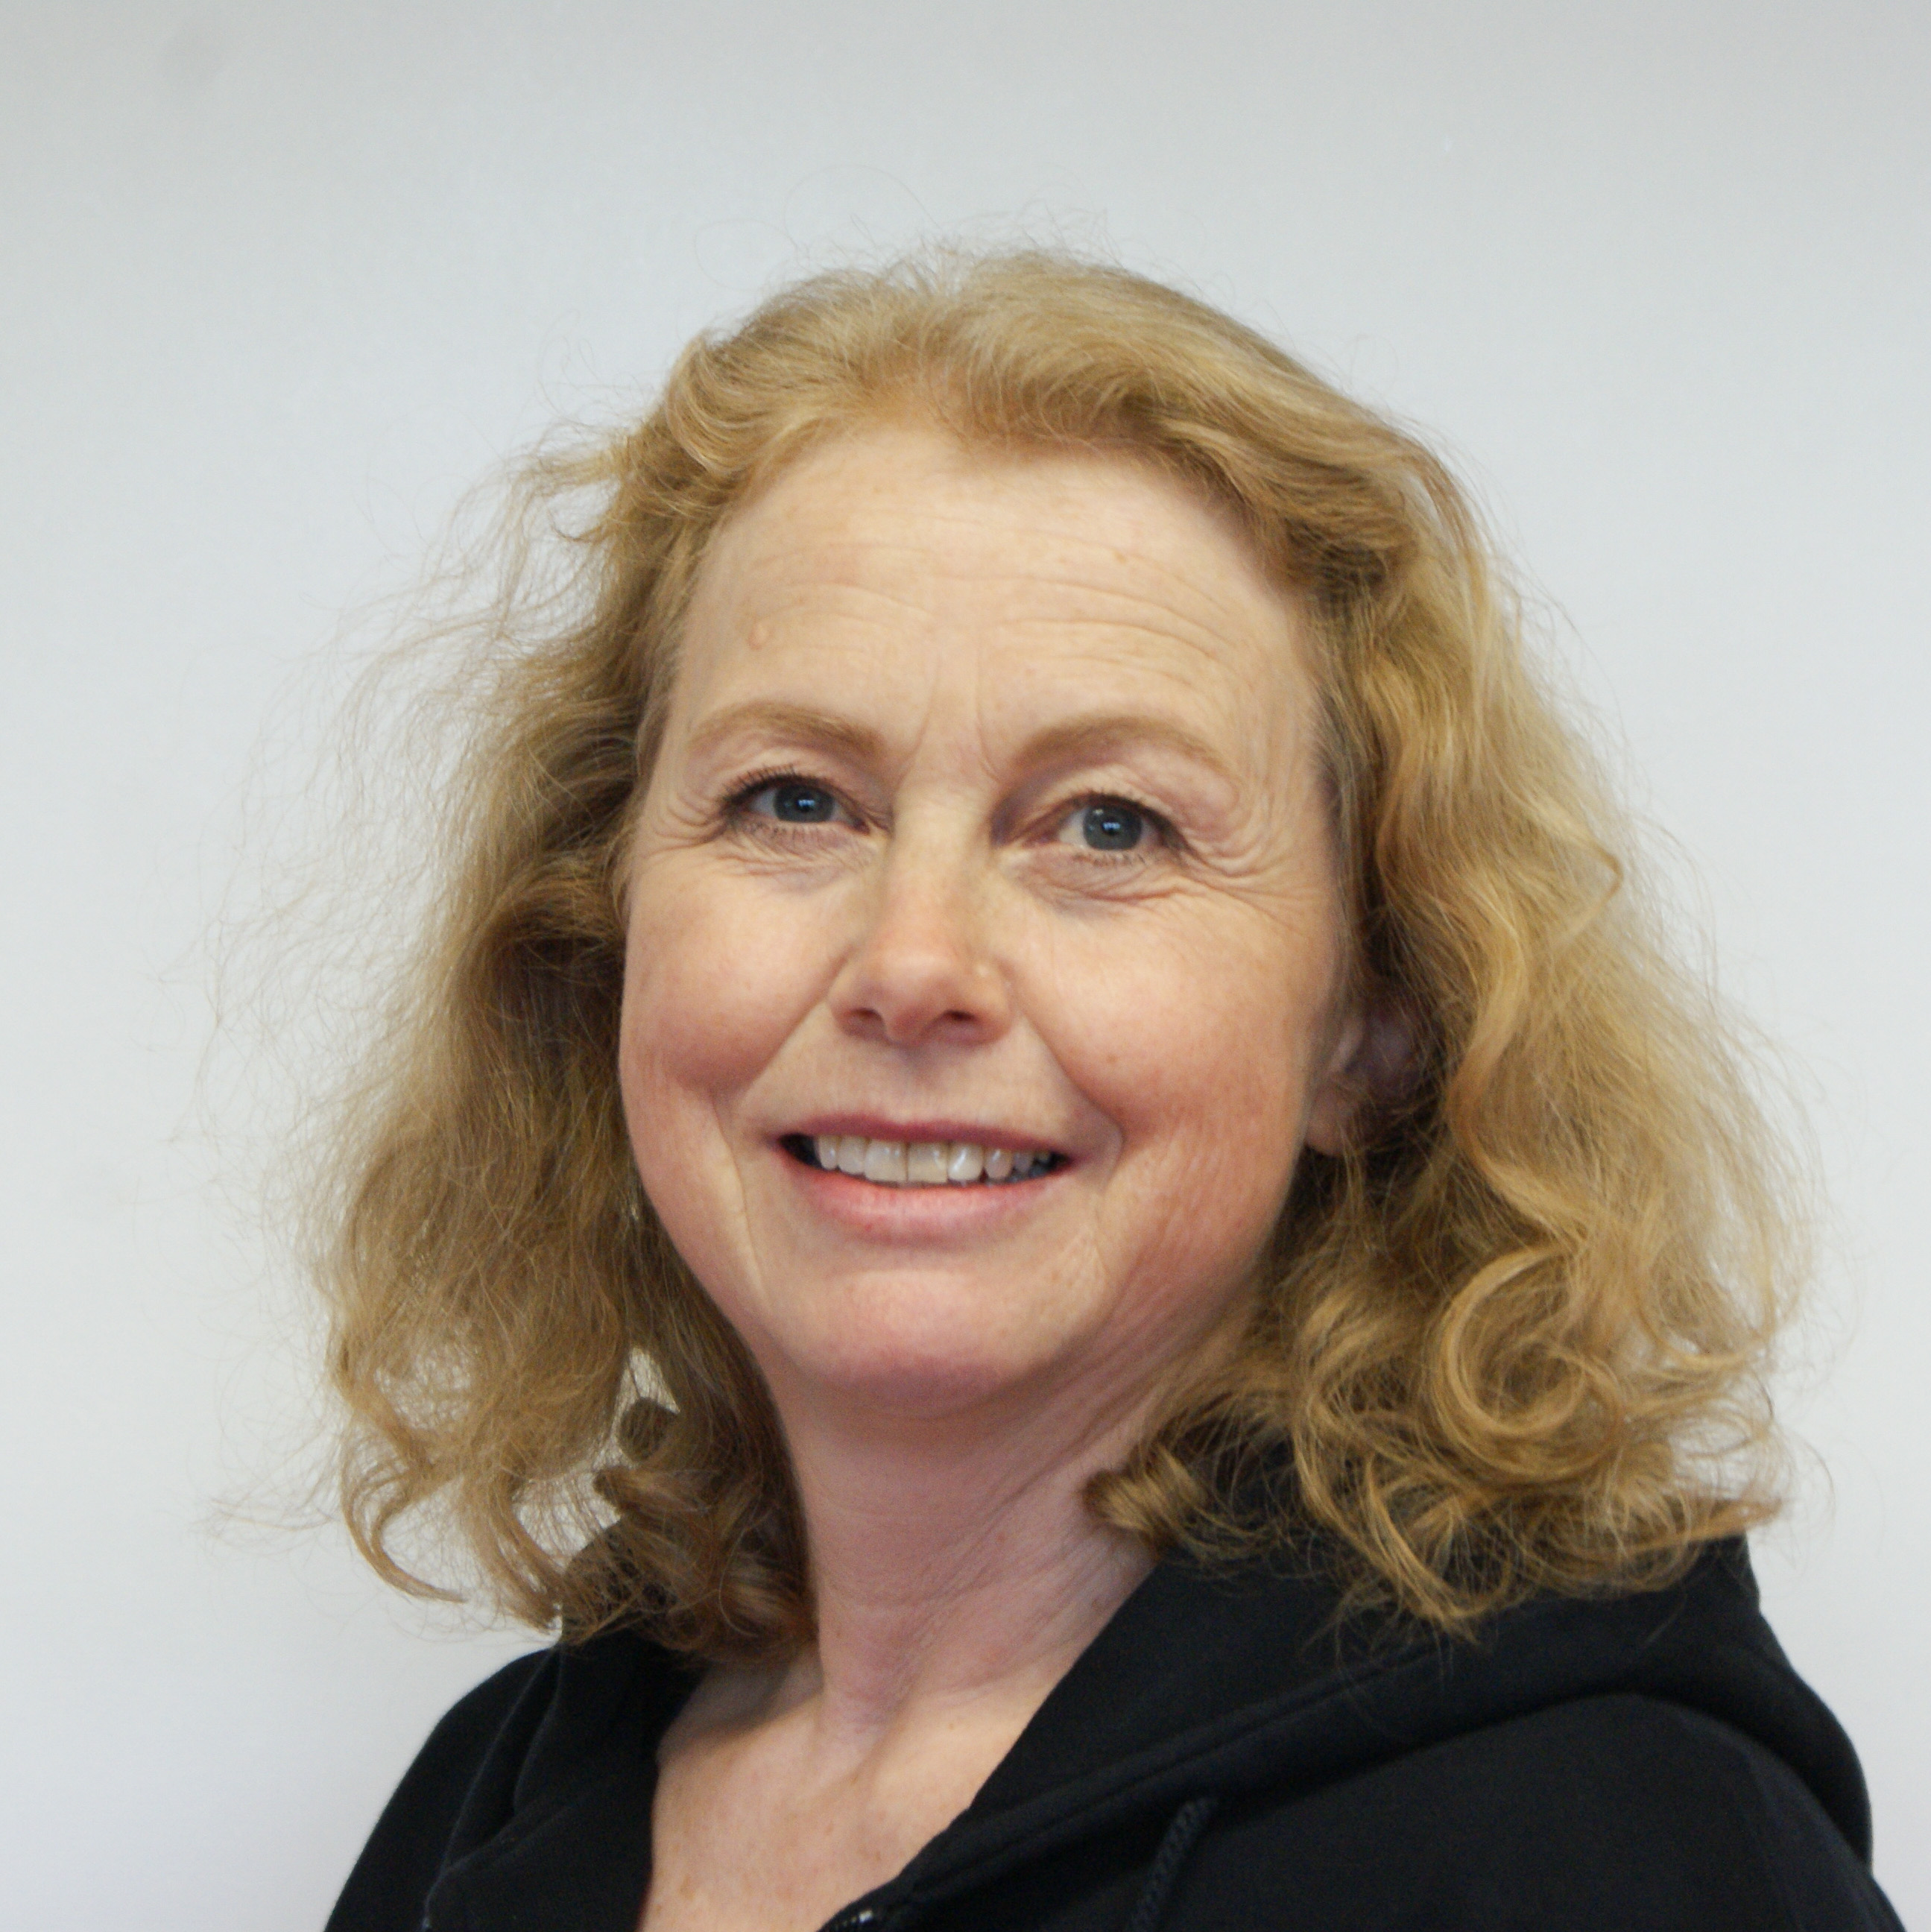
\includegraphics[width=.95\textwidth]{GiselaLehner.jpg}}
\end{minipage}
\hfill
\begin{minipage}[t]{0.6\textwidth}
\vspace{0pt}
\singlespacing
\Large{Trainerin}\\
\huge{\textbf{Gisela Lehner}} \par
\flushright
\normalsize{\textit{\textrm{``Leben ist Bewegung - Also nur nicht müde werden!''}}}
\end{minipage}
%\end{figure}

\vspace*{\fill}
\begin{minipage}[t]{0.35\textwidth}
\vspace{0pt}
\flushleft
Ausbildungen
\end{minipage}
\hfill
\begin{minipage}[t]{0.6\textwidth}
\vspace{0pt}
\onehalfspacing
Fitnesstrainer A-Lizenz (DOSB)\\
Fitnesstrainer B-Lizenz (BGKV)\\
Fitnesstrainer C-Lizenz (BGKV)\\
\end{minipage}

\vspace{1cm}
\begin{minipage}[t]{0.35\textwidth}
\vspace{0pt}
\flushleft
Hobbys
\end{minipage}
\hfill
\begin{minipage}[t]{0.6\textwidth}
\vspace{0pt}
\onehalfspacing
Reisen\\
Literatur\\
Musik\\
Fitness
\end{minipage}

\vspace*{\fill}
\begin{minipage}[t]{0.45\textwidth}
\vspace{0pt}
\onehalfspacing
\footnotesize{FC Puchheim e.V. \\ Fitness-Studio \\ Abteilung Kraft \& Fitness}
\end{minipage}
\hfill
\begin{minipage}[t]{0.45\textwidth}
\vspace{0pt}
\flushright

\includegraphics[width=1.5cm]{FCPlogo.png}
\end{minipage}
\vspace{1cm}


\end{document}
